\subsection{$^{10}$Be Konzentration}


Im letzten Versuchsteil soll die Konzentration des radioaktiven $^{10}$Be in den Proben KY (siehe Auswertung im Niedrigenergiebereich) berechnet werden.
Diese wird berechnet als Verhältnis der Zählraten im Ionisations Detektor und der des stabilen Isotopes $^9$Be im Faraday-Cup.
Da beide Detektoren die Strahlen unter Umständen nicht mit gleicher Effizienz detektieren, ist es notwendig eine Vergleichsmessung einer Probe mit bekannten Isotopenverhältnis durchzuführen.
Mit dieser Messung wird ein Normalisierungsfaktor $f_{norm}$ ermittelt, welcher auf die Messung angewandt werden kann, um das Verhältnis zu ermitteln.
Dieser berechnet sich zu:
\[
f_{norm} = \frac{r_{nominal, ref}}{r_{meas, ref}} = \frac{1,704 \cdot 10^{-12}}{8,964 \cdot 10^{-13}} = 1,900
\]
hier ist $r_{nominal, ref}$ das bekannte Verhältnis der Isotope und $r_{meas, ref}$ das gemessene Verhältnis.
Das Verhältnis der Isotope in der gemessenen Probe ergibt ($r_{real, sample}$) sich damit zu:
\[
r_{real, sample} = r_{meas, sample} \cdot f_{norm}
\]
mit dem gemessenen Verhältnis ($ r_{meas, sample}$).
Die Konzentration des Radionuklides berechnet sich damt zu:
\begin{equation}
c_{sample} = r_{real, sample} \cdot \frac{m_{spike}}{M_{sample}}
\end{equation}
mit der Masse der Probe $M_{sample}$ und der Menge des stabilen Isotops $m_{spike}$.
Die gemessenen Werte der Proben und die berechneten Konzentrationen sind in Tab. \ref{concentrations} zu finden.

\begin{table}[h]
\centering
\caption{Gemessene Werte zur Berechnung der $^{10}$Be Konzentration in den Proben.}
\begin{tabular}{|c |c| c|c|c|}
\hline
Probe& $M_{sample}$[g] & $m_{spike}$ [g] & $ r_{meas, sample}$ & $c_{sample}$ \\
\hline
KY13 & $14,692$ &  $3,11 \cdot 10^{-4}$ & $ (4,15 \pm 0,19)\cdot 10^{-13}$ &     $(1.668 \pm 0,076) \cdot 10^{-17}$ \\
KY14 & $16,775$ &  $3,09 \cdot 10^{-4}$ & $ (4,11 \pm 0,19)\cdot 10^{-13}$ &     $(1,438 \pm 0,066) \cdot 10^{-17}$ \\
KY16 & $16,586$ &  $3,05 \cdot 10^{-4}$ & $ (3,28 \pm 0,15)\cdot 10^{-13}$ &     $(1,146 \pm 0.054) \cdot 10^{-17}$ \\
KY17 & $9,489  $ &  $3,04 \cdot 10^{-4}$ & $ (1,533 \pm 0,081)\cdot 10^{-13}$ & $(9,330 \pm 0.049) \cdot 10^{-17}$ \\
\hline
\end{tabular}
\label{concentrations}
\end{table}

In Abb. \ref{deep} wurden diese Konzentrationen über die mittlere Tiefe der Proben geplottet.
Wir können sehen dass diese, innerhalb ihrer Messgenaugkeit, näherungsweise linear abfällt.
Eine Abnahme ist prinzipiell auch zu erwarten gewesen, da $^{10}$Be vor allem durch Ereignisse mit kosmischer Strahlung entsteht.
Tieferliegende Schichten in den Proben sind entsprechend stärker von dieser Abgeschirmt, weshalb dort weniger $^{10}$B produziert wird.
Nach dieser Argumentation würde man jedoch eine exponentielle Abnahme der Konzentration erwarten.
Eine solche wird hier nicht direkt beobachtet, kann aber bei nur vier Messpunkten auch nicht ausgeschlossen werden.
Für ein besseres Ergebniss würden sicherlich mehr Proben, also mehr Messpunkte, sorgen.
Unter Umständen spielen hier auch andere Prozesse eine Rolle, welche die Produktionsraten von$^{10}$B verändern.
Dafür wäre jedoch eine Neutronenquelle notwendig, welche $^{10}$B durch Neutroneneinfang erzeugen könnte.
Eine solche innerhalb der Proben wurde zwar nicht untersucht, kann aber als unwahrscheinlich angenommen werden.

\begin{figure}[ht]
  \centering
  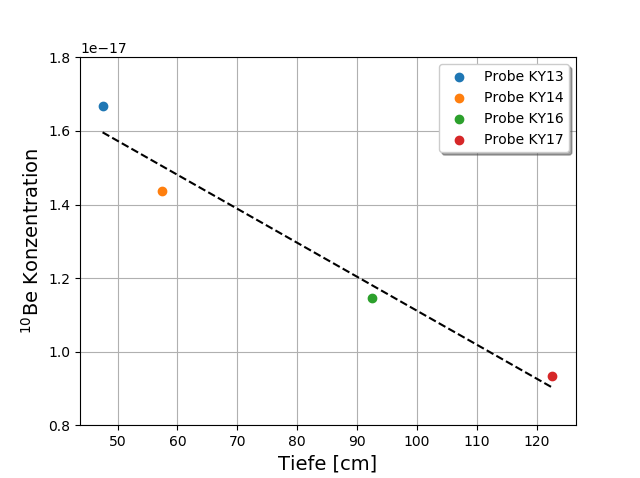
\includegraphics[width=0.7\linewidth]{Pictures/10be_konzentration.png}
  \caption{Berechnete Konzentration von $^9$Be in den Proben in Abhängigkeit von der Tiefe innerhalb der Probe, mit linearen Fit.}
  \label{deep}
\end{figure}
\clearpage
